\documentclass[french]{article}
\usepackage[utf8]{inputenc}
\usepackage[T1]{fontenc}
\usepackage{lmodern}
\usepackage[a4paper]{geometry}
\usepackage{babel}

\usepackage{color}
\usepackage{epsfig}

\newcommand{\figref}[1]{Figure~\ref{#1}}
\newcommand{\algref}[1]{Algorithm~\ref{#1}}
\newcommand{\theoremref}[1]{Theorem~\ref{#1}}
\newcommand{\lemmaref}[1]{Lemma~\ref{#1}}
\newcommand{\defref}[1]{Definition~\ref{#1}}
\newcommand{\secref}[1]{Section~\ref{#1}}
\newcommand{\tabref}[1]{Table~\ref{#1}}

% % % % % % % % % % % % % % % % % % % % % % % % % % % % % % % % % % % % % %
\begin{document}
\title{Building genetically inspired constraints \\
with the Parsimony framework}
\author{}
\maketitle
\begin{abstract}
\end{abstract}



% % % % % % % % % % % % % % % % % % % % % % % % % % % % % % % % % % % % % %
\section{Les données et les contraintes}
\subsection{Websters et résultats univariés}
Données décrites dans les papiers \cite{Myers2007, Webster2009}.
Voir aussi le rapport de V Guillemot sur l'étude que nous avions faite pour se caler sur le papier séminal de 2009 concernant l'association avec le GE.

Les données contiennent des SNPs, de l'expression de gène et le statut clinique pour 380 (TOFIX) personnes. pour l'expression, des données considérées sont les celles de l'article qui supprime les effets confondants (statut Apo, TOFIX). Pour la regression logistique on considère le statut (Alz, Ctl). Pour la régression linéaire on considère l'expression du gène KIF1B qui ressort dans le papier comme gène s'associant avec des SNPs en univarié lorsque la maladie est avérée : l'interprétation exacte du papier \cite{Webster2009} est très difficile !

\subsection{Contraintes}
Les contraintes considérées sont de plusieurs natures :
\subsection{Contraintes de groupes}
Rendues par du GroupLasso. 
On considère les informations :
\begin{itemize}
	\item  GeneOntology (group avec overlap massif car en tant qu'ontologie il s'agit de groupe organisés hiérarchiquement),
	\item pathway Keggs ou autre base de collection de gènes : c'est aussi du group avec overlap. Cette base est utilisée par Montana et coll. \cite{Silver2012} et aussi par Chen et coll. \cite{Chen2010}
\end{itemize}

On pourrait considérer la prise en compte d'une contrainte de type fused lasso (flou pour ce qui me concerne).

\subsection{Contraintes de régions recombinantes}
Il s'agit de rendre compte de la plus ou moins grande probabilité de recombinaison observée sur le génome. Les zones à faible probabilité pourraient être traitées avec une approche Group-TV : de la cohérence serait demandée dans de telles régions.

La description des données de probabilité de recombinaison est donnée dans 

% % % % % % % % % % % % % % % % % % % % % % % % % % % % % % % % % % % % % %
\section{Travaux en cours}
\subsection{Approches GL}

Les pénalités travaillées sont Ridge + L1 dans le cas de la regression logistique.
\begin{itemize}
\item Montage des contraintes repose sur inst\_bioresource OK pour gene et snp tedious pour les pathways
\item Mise en place d'une visu des résultats
\item \textcolor{red}{Mise en place d'un cadre pour le choix des hyperparametres. Map Reduce et usage de Gabriel}
\item \textcolor{red}{passage a l'échelle pour le nombre de pathways}
\item \textcolor{red}{Choix des poids a appliquer à chacun des pathway. ici il y a une ambiguité explicitée dans la \figref{fig:fig_group} }
\end{itemize}

\begin{figure}[!!!h]
    \begin{center}
        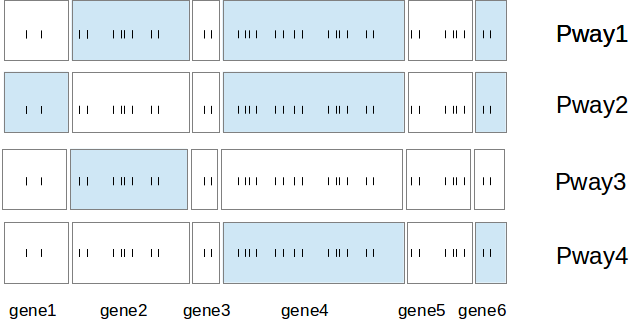
\includegraphics[width=0.8\textwidth]{{{images/fig_group}}}
        \caption{Illustration de la difficulté du choix des poids pour un pathway donné. Les régions bleus dans un pathway sont les gènes qui sont gardés. Les SNPs sont les petits bâtons. Pour un pathway de meme longueur il peut etre consitué de gènes plus ou moins long. Il semble que les pathways contenant des gènes longs sont favorisés.}
        \label{fig:fig_group}
    \end{center}
\end{figure}



\bibliographystyle{plain}
\bibliography{genomic_constraint}
\end{document}
